\documentclass[a4paper, 12pt]{article}
\usepackage{listings}
\usepackage{pdfpages}
\usepackage{caption}
\usepackage[ngerman]{babel}
\usepackage{float}
\usepackage[backend=biber]{biblatex}
\usepackage{csquotes}
\usepackage{abstract}
\usepackage{graphicx}
\addbibresource{Literatur.bib}
\begin{document}

\begin{titlepage}
	\centering
	{\scshape\Large Maturitätsarbeit an der Kantonsschule Zürich Nord \par}
	\vspace{1cm}
	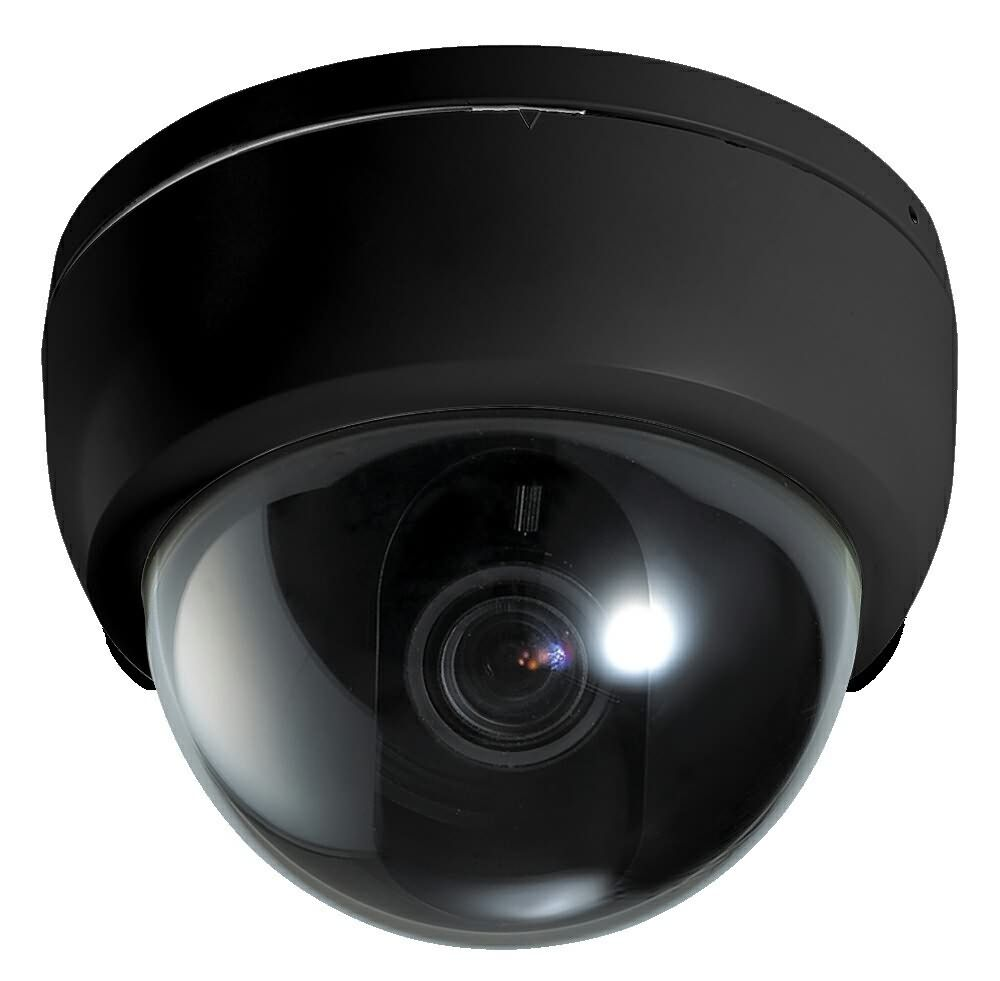
\includegraphics[width=0.3\textwidth]{Ueberwachungskamera}\par\vspace{1cm}
	\vspace{1cm}
	{\LARGE Programmieren einer Software für das Erkennen der Farbe eines Rubik's Cubes\par}
	\vspace{2cm}	
	{\Large\itshape Leon Erzberger\par}
	
	{\large M6d\par}
	\vfill
	Betreuungsperson\par
	David \textsc{Tyndall}

	\vfill

% Bottom of the page
	{\large Zürich, Dezember 2019\par}
\end{titlepage}
\pagenumbering{Roman}

\lstset{ numbers=left, basicstyle=\footnotesize, breaklines, tabsize=2, literate={\ \ }{{\ }}1}
\begin{abstract}%
\noindent
Ziel dieser Maturaarbeit war, ein möglichst gutes Programm für die Farberkennung eines Rubik's Cubes zu programmieren. Dafür wurden die beiden Farbräume RGB und HSV miteinander verglichen. Ausserdem wurde eine spezielle Methode für das Erkennen von schwarzen und weissen Feldern ausprobiert. Zum Schluss wurden dann noch zwei Methoden verglichen, die Korrekturen vornahmen, so dass jede Farbe exakt 9 mal vorkommt. Das ausschliessliche Verwenden von Hue zur Unterscheidung der Farben, das Benützen von der Methode, um weiss und schwarz loszuwerden, und das Verwenden einer der zwei Korrekturmethoden lieferte die besten Ergebnisse, mit durchschnittlich 8.5 Fehlern bei 54 Feldern.
\end{abstract}
\tableofcontents
\clearpage
\pagenumbering{arabic} 
\newpage
\section{Einleitung}
In dieser Arbeit wurde versucht, eine Software zu programmieren, die einen Rubik's Cube möglichst gut erkennen soll. Dabei werden Probleme untersucht, die im Gebiet der Farberkennung auftreten können. Dabei werden verschiedene Lösungsansätze miteinander verglichen und es wird erklärt, wie sie im Code angewendet wurden.
\subsection{Rubiks Cube}
Um die Farben eines Rubiks Cubes zu erkennen, muss erst einmal klar sein, wie er überhaupt aufgebaut ist. Ein Rubik's Cube (im Folgenden Würfel genannt) besteht aus 26 Steinen. Diese sind in einer 3x3x3-Würfelform angeordnet, in der der Mittlere Würfel fehlt. Die Steine sind so mit sechs verschiedenen Farben gefärbt, dass jede Seite des Würfels eine Farbe hat (vgl. Abbildung 1). Dabei existieren insgesamt sechs Mittelsteine, auf jeder Seite einer, die je eine einzige gefärbte Fläche (im Folgenden Mitte genannt) haben. Diese Mitten haben jeweils eine der sechs Farben. Sie ändern beim Verdrehen des Würfels ihre relative Position zueinander nicht. Neben den Mittelsteinen gibt es auch noch Seitensteine. Diese haben jeweils zwei oder drei gefärbte Flächen. So eine Fläche wird im Folgenden "`Seite"' genannt.
\begin{figure}[H]
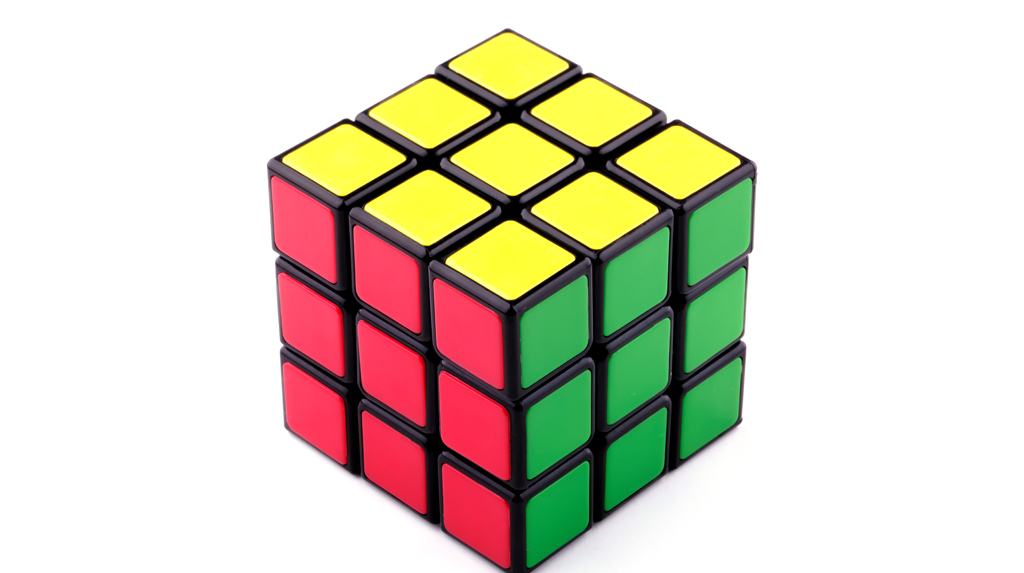
\includegraphics[scale=1.5]{Wuerfel_Billd}
\caption{Gelöster Rubik's Cube mit einer Farbe pro Seite. \cite{Wuerfelbild}}
\end{figure}
\subsection{Grundlegende Idee}
Die grundliegende Idee ist die, dass der Rubik's Cube immer an einem Fixen Punkt festgemacht wird, und dann von zwei gegenüberliegenden Kameras fotografiert wird (vgl. Abbildung 2). So sind die Felder des Würfels immer an der gleichen Stelle im Bild, und es braucht keine Mustererkennung, um die Felder zu finden. Um die Felder dann einer Farbe zuzuordnen, werden keine im vorderein definierten Farben verwendet, sondern es werden die Farbwerte der Mittelsteine herausgelesen, und die restlichen Felder werden dann diesen zugeordnet. So wird vermieden, dass man bei jedem neuen Würfel, der andere Farben besitzt, wieder mühselig die richtigen Farbwerte suchen muss, um die Definitionsbereiche zu erstellen. Wenn ausserdem die Lichtverhältnisse  mal etwas dunkler oder heller sind, wird dies dann automatisch miteinberechnet, da die Mitten dann auch dunkler sind. 
\begin{figure}[H]
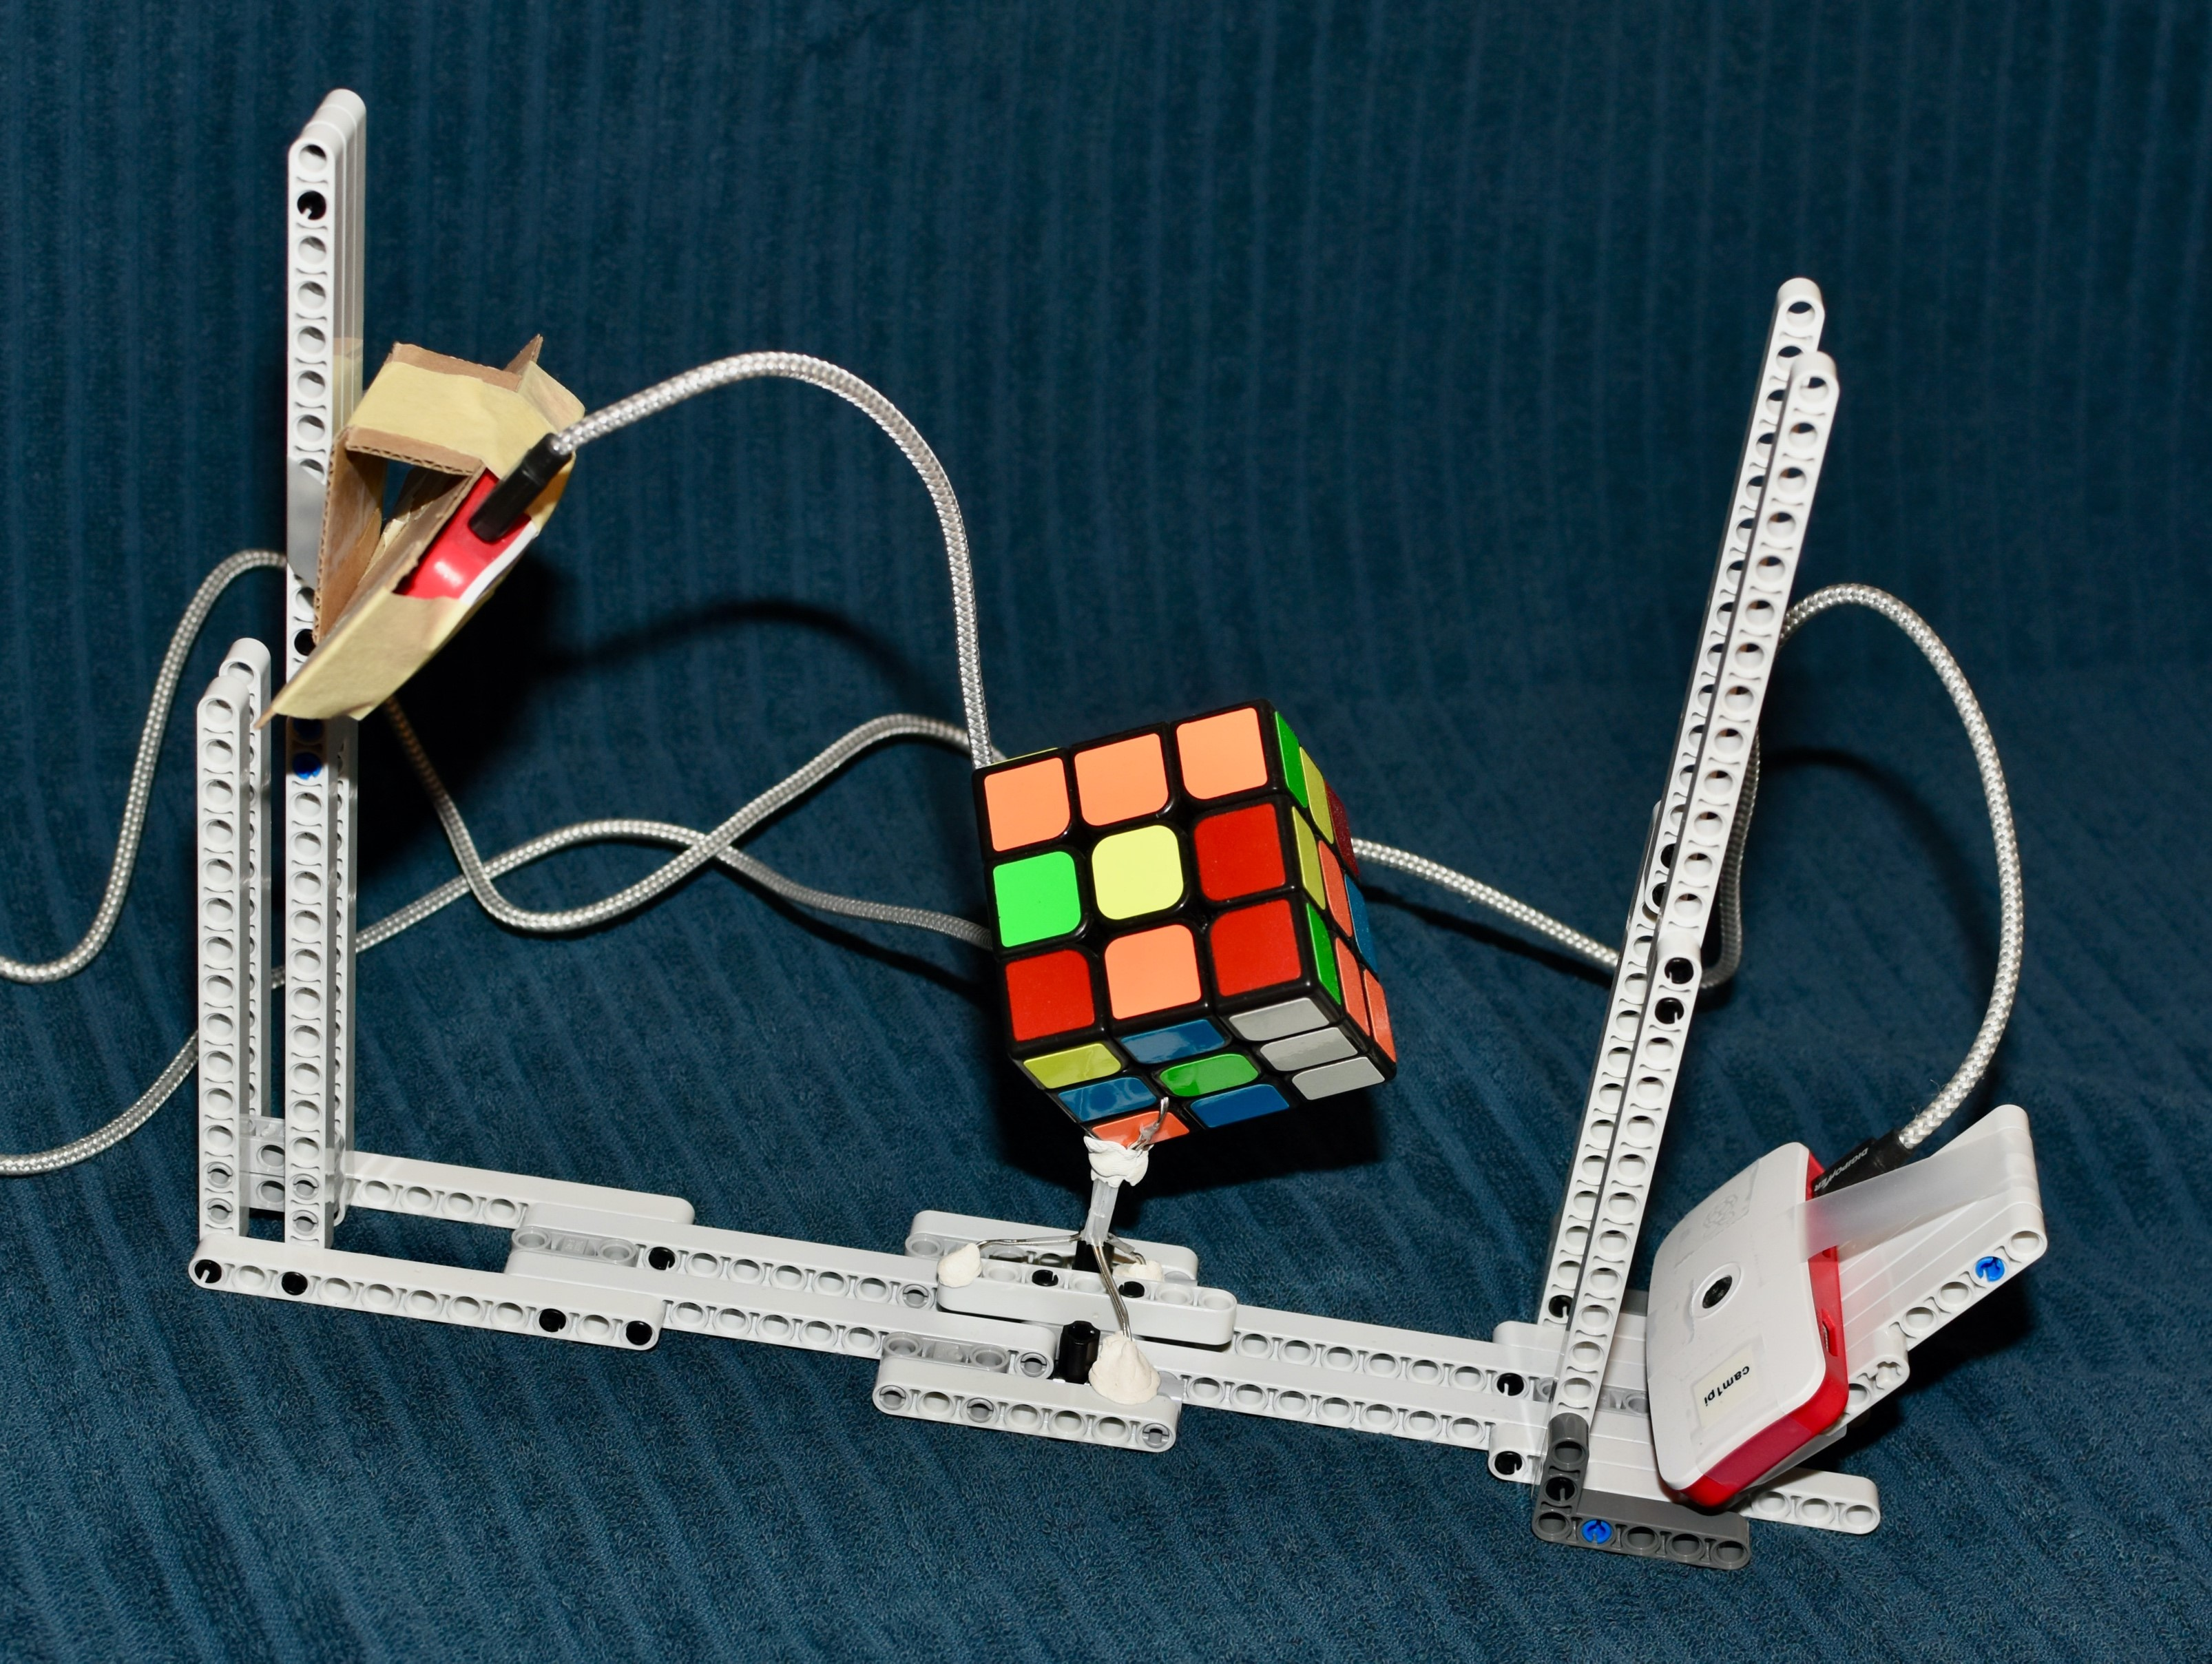
\includegraphics[scale=0.25]{Aufbau_Bild}
\caption{Aufbau, um Rubik's Cube immer vom gleichen Winkel aus zu fotografieren.}
\end{figure}
\newpage
\section{Umsetzung und Resultate}
\subsection{Farbräume}
Zuallererst musste festgelegt werden, wie die Farben der Steine aus dem Bild ausgelesen werden. Dafür muss man zuerst verstehen, wie Farben auf einem Bild überhaupt dargestellt werden. Dies geschieht auf einem Computer mithilfe eines Farbraumes. Ein Farbraum ist eine fest definierte Anzahl an Farben, die oft mithilfe von drei Variablen beschrieben werden. Eine Bilddatei enthält somit nur Farben, die durch eine Kombination der drei Variablen erstellt werden kann. \cite{Farbraum} Diese Variablenwerte können dann ohne Probleme ausgelesen und miteinander verglichen werden. Zwei der gängigsten Farbräume, die hier miteinander verglichen werden, sind der RGB- und der HSV-Farbraum. 
\subsubsection{RGB}
RGB ist der Standard-Farbraum, für die digitale Bildwiedergabe. Er setzt sich aus drei Werten für Rot, Grün, und Blau zusammen. Die Werte gehen jeweils von 0 bis 255, wobei die Farbe bei 0 nicht vorhanden ist, und bei 255 die Farbe mit voller Intensität leuchtet. (0, 0, 0) ist somit schwarz und (255, 255, 255) ist weiss. Der gesamte Farbraum lässt sich als Würfel in einem Koordinatensystem darstellen, wobei die Achsen jeweils die Intensität einer Farbe beschreiben (vgl. Abbildung 3).
\begin{figure}[H]
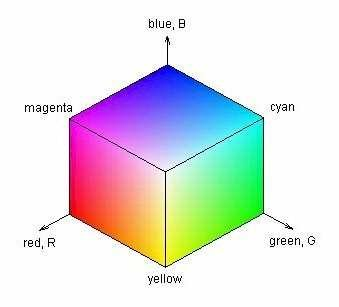
\includegraphics[scale=0.5]{RGB_Wuerfel}
\caption{RGB-Farbraum in einem Koordinatensystem visualisiert mit Achsen für rot, grün und blau. \cite{RGBBild}}
\end{figure}
 Der RGB-Farbraum ist ein additiver Farbraum. Das bedeutet, dass bei nichts angefangen wird, und je höher die Werte werden, desto mehr Farbe vorhanden ist. \cite{RGBHSV} Deshalb wird RGB auch bei vielen Arten von Beleuchtung verwendet, wie Fernseher und Computerbildschirme, die ihre Pixel mit roten, grünen und blauen LEDs beleuchten. Auch der Mensch erkennt Farben auf diese Weise, da im Auge Rezeptoren vorhanden sind, die empfindlich auf die Wellenlängen von Rot, Grün und Blau sind.
\subsubsection{HSV}
Der HSV-Farbraum setzt sich aus den Werten "`Hue"', "`Saturation"' und "`Value"' zusammen. Hue ist ein Wert für den Farbton, und geht standardmässig von 0 bis 179. Ausserdem ist der Wertebereich von Hue kreisförmig, was heisst, dass 0 und 179 nebeneinander sind und es somit kein Anfang oder Ende gibt. "`Saturation"' beschreibt die Sättigung und Intensität der Farbe und geht von 0 bis 255, wobei 0 keine Sättigung und somit Weiss bedeutet und bei 255 die Farbe vollends vorhanden ist. "`Value"' ist ein Mass für die Helligkeit und reicht ebenfalls von 0 bis 255. Wenn der Value bei null ist, dann spielt es keine Rolle was der Farbton ist, und die Farbe wird schwarz. Je höher der Value dann geht, desto heller wird die Farbe. \cite{RGBHSV} Der HSV-Farbraum wird häufig in Form eines Zylinders visualisiert (vgl. Abbildung 4).
\begin{figure}[H]
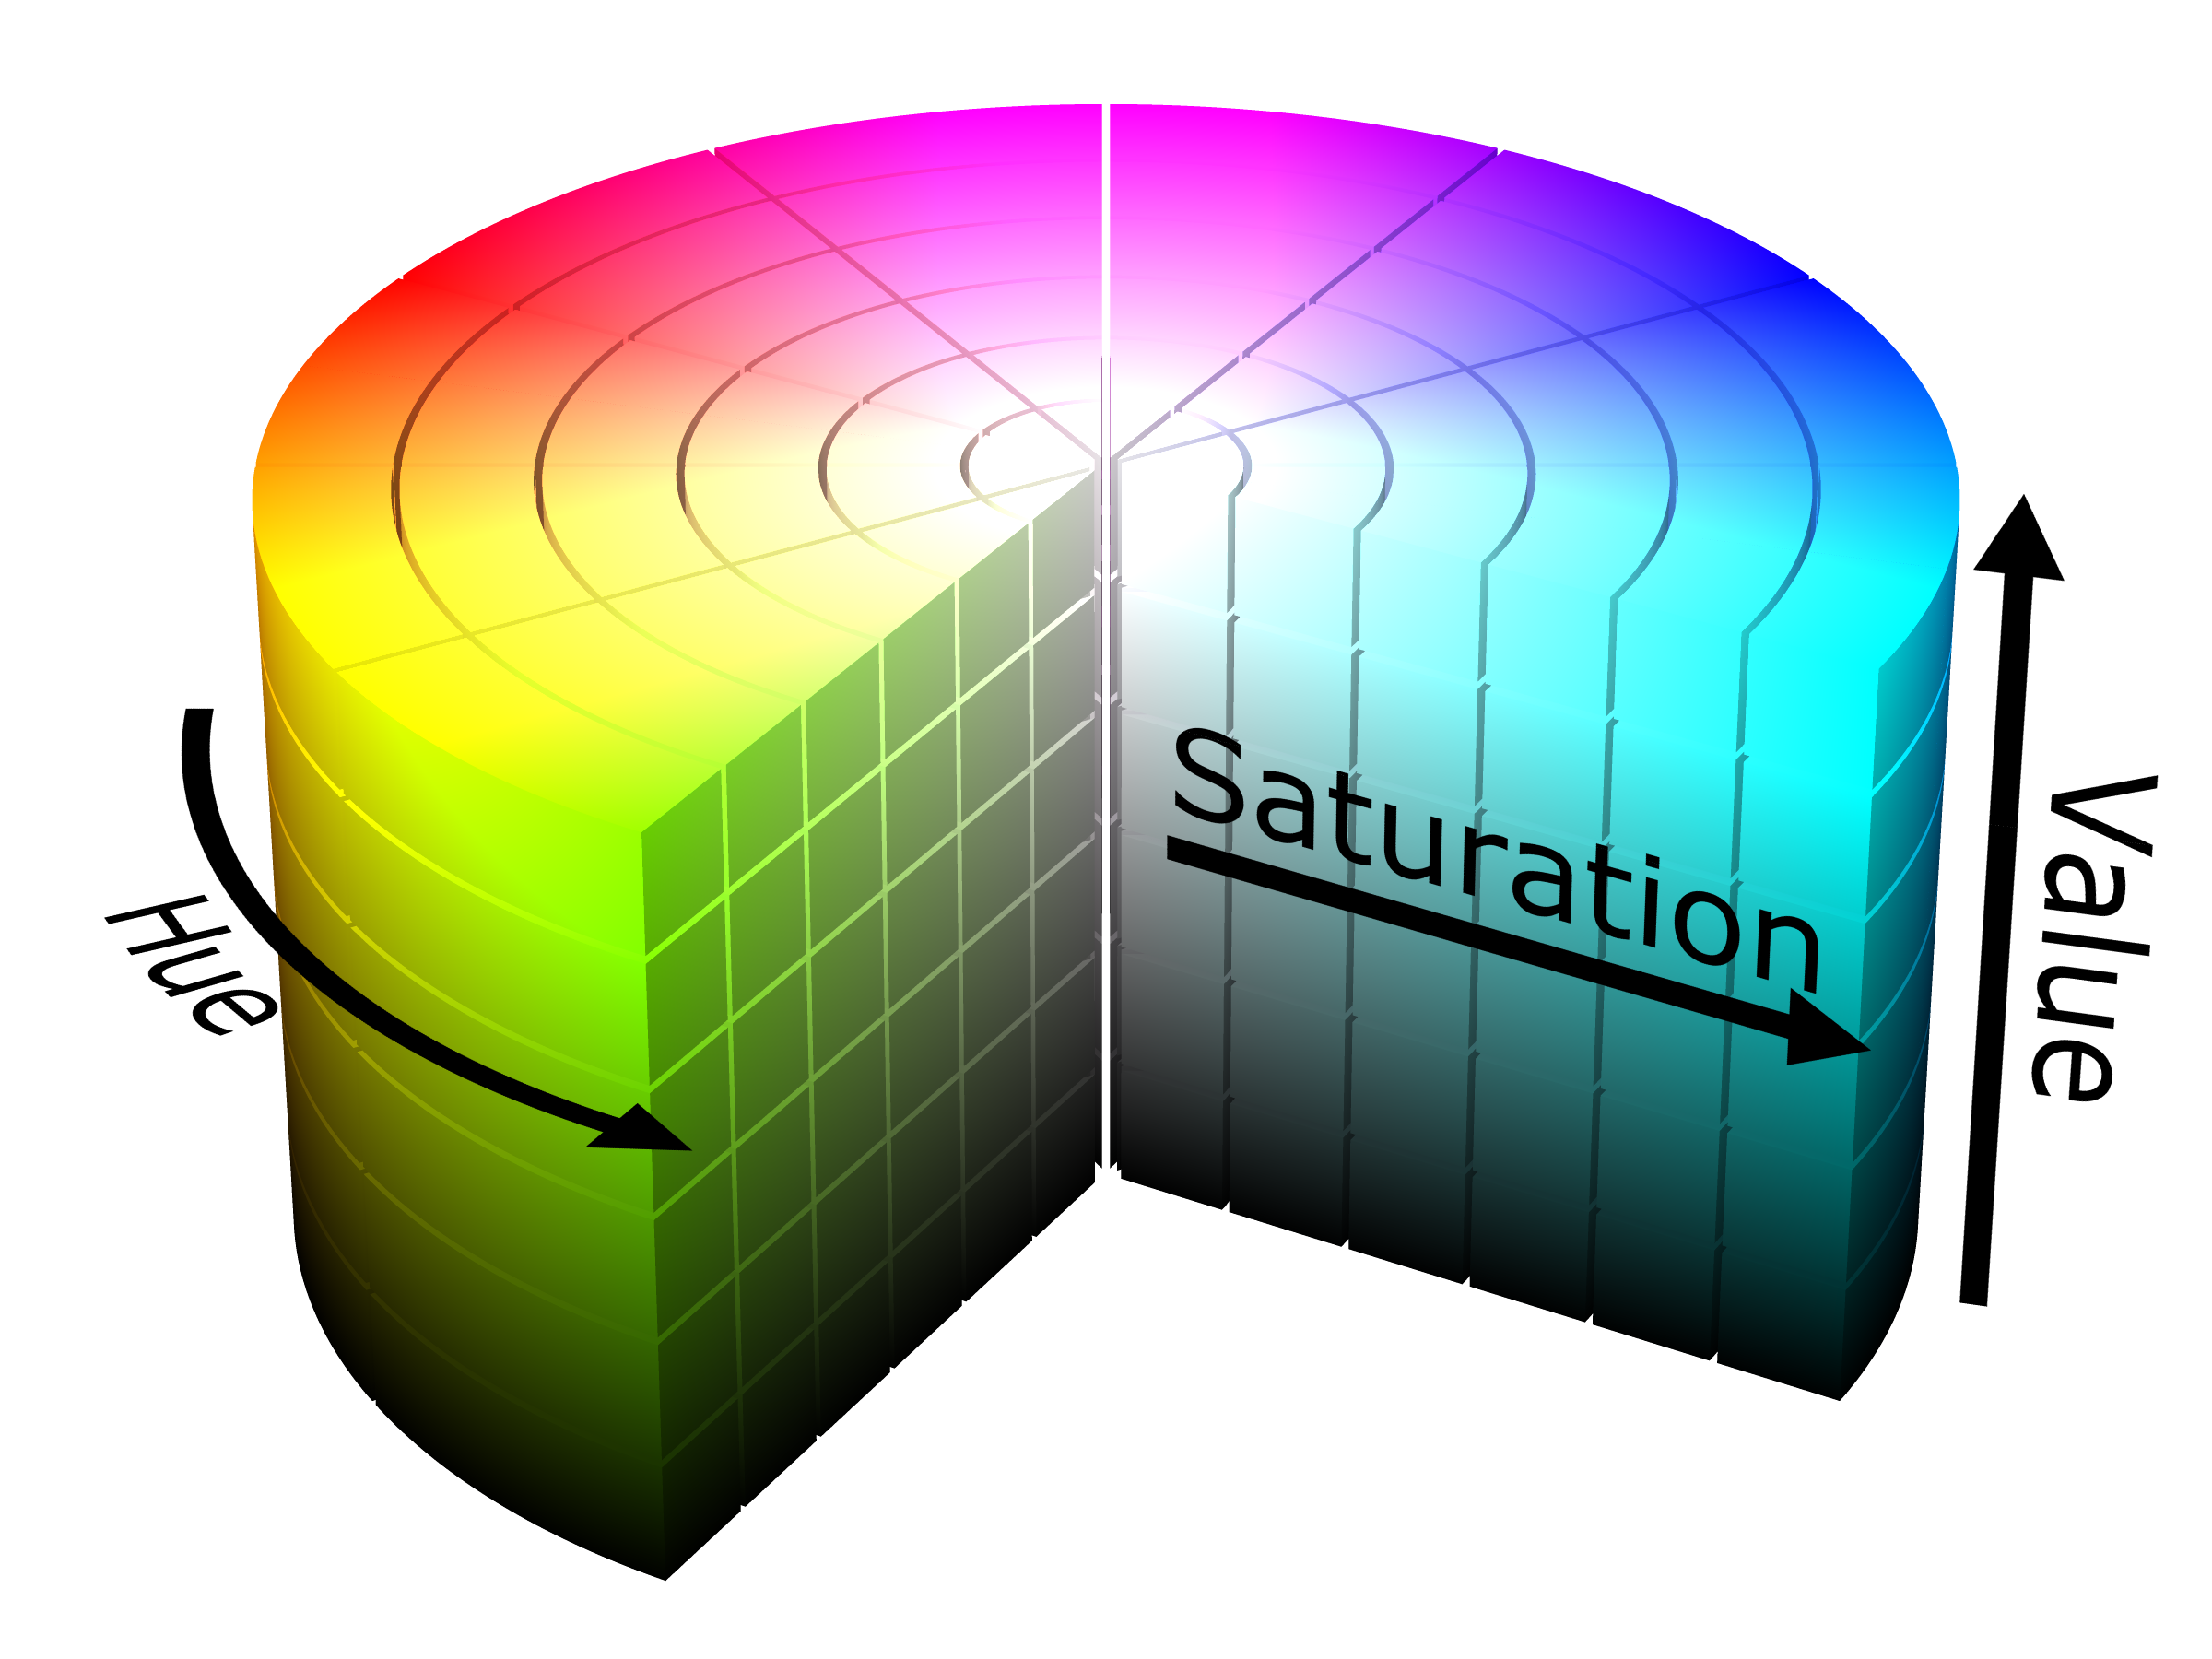
\includegraphics[scale=0.07]{HSV_Zylinder} 
\caption{HSV-Farbraum als Zylinder visualisiert mit Saturation als Radius, Value als Höhe und Hue als Winkel. \cite{RGBHSV}}
\end{figure}
\subsubsection{Anwendung im Code}
Zuerst werden für jedes Feld auf dem Würfel die RGB-Werte von 400 Pixeln in einem 20x20-Quadrat ausgelesen. Danach werden die Durchschnitte davon berechnet und in einer Liste gespeichert.
\lstinputlisting[language=Python, linerange={2-7}, caption={Auslesen der RGB-Werte der Felder des Rubik's Cubes.}, captionpos=b]{listings.py}
Als nächstes werden die Seiten einer Mitte zugeordnet. Dafür wird in Zeile 2 für jede Seite eine Schleife initiiert, die die 6 Mitten durchgeht. Für jede Mitte wird nun der Abstand zur Seite im verwendeten Farbraum berechnet. Da RGB ein Farbraum mit kartesischen Koordinaten ist, kann der Abstand mit Hilfe des Satzes des Pythagoras berechnet werden. Somit kann man die Differenzen zwischen den R-, G-, und B-Werten einzeln berechnen und danach die Quadrate davon addieren. Dies geschieht in den Zeilen 5 und 6. Danach wird in Zeile 7 die Wurzel davon gezogen und in einer Liste abgespeichert. In den Zeilen 8-10 wird schliesslich evaluiert, welche Mitte am nächsten ist, und die Seite wird dieser zugeordnet. 
\lstinputlisting[language=Python, linerange={10-19}, caption={Zuordnung der Seiten zu einer Mitte.}, captionpos=b]{listings.py}
\subsubsection{Vergleich}
Jetzt, wo die Farbräume und Methodik der Zuordnung klar sind, stellt sich die Frage, was die besten Ergebnisse liefert. Hierfür wurden fünf Ideen ausprobiert:
\begin{enumerate}
  \item Die RGB-Werte verwenden
  \item Die HSV-Werte verwenden
  \item Nur Hue und Saturation verwenden
  \item Nur Hue und Value verwenden
  \item Nur Hue verwenden
\end{enumerate}
Diese fünf Methoden wurden alle auf zehn Bilder von Rubiks Cubes angewandt, und anschliessend wurde ermittelt, wie viele Fehler die Methoden im Schnitt hatten. 
\begin{figure}[H]
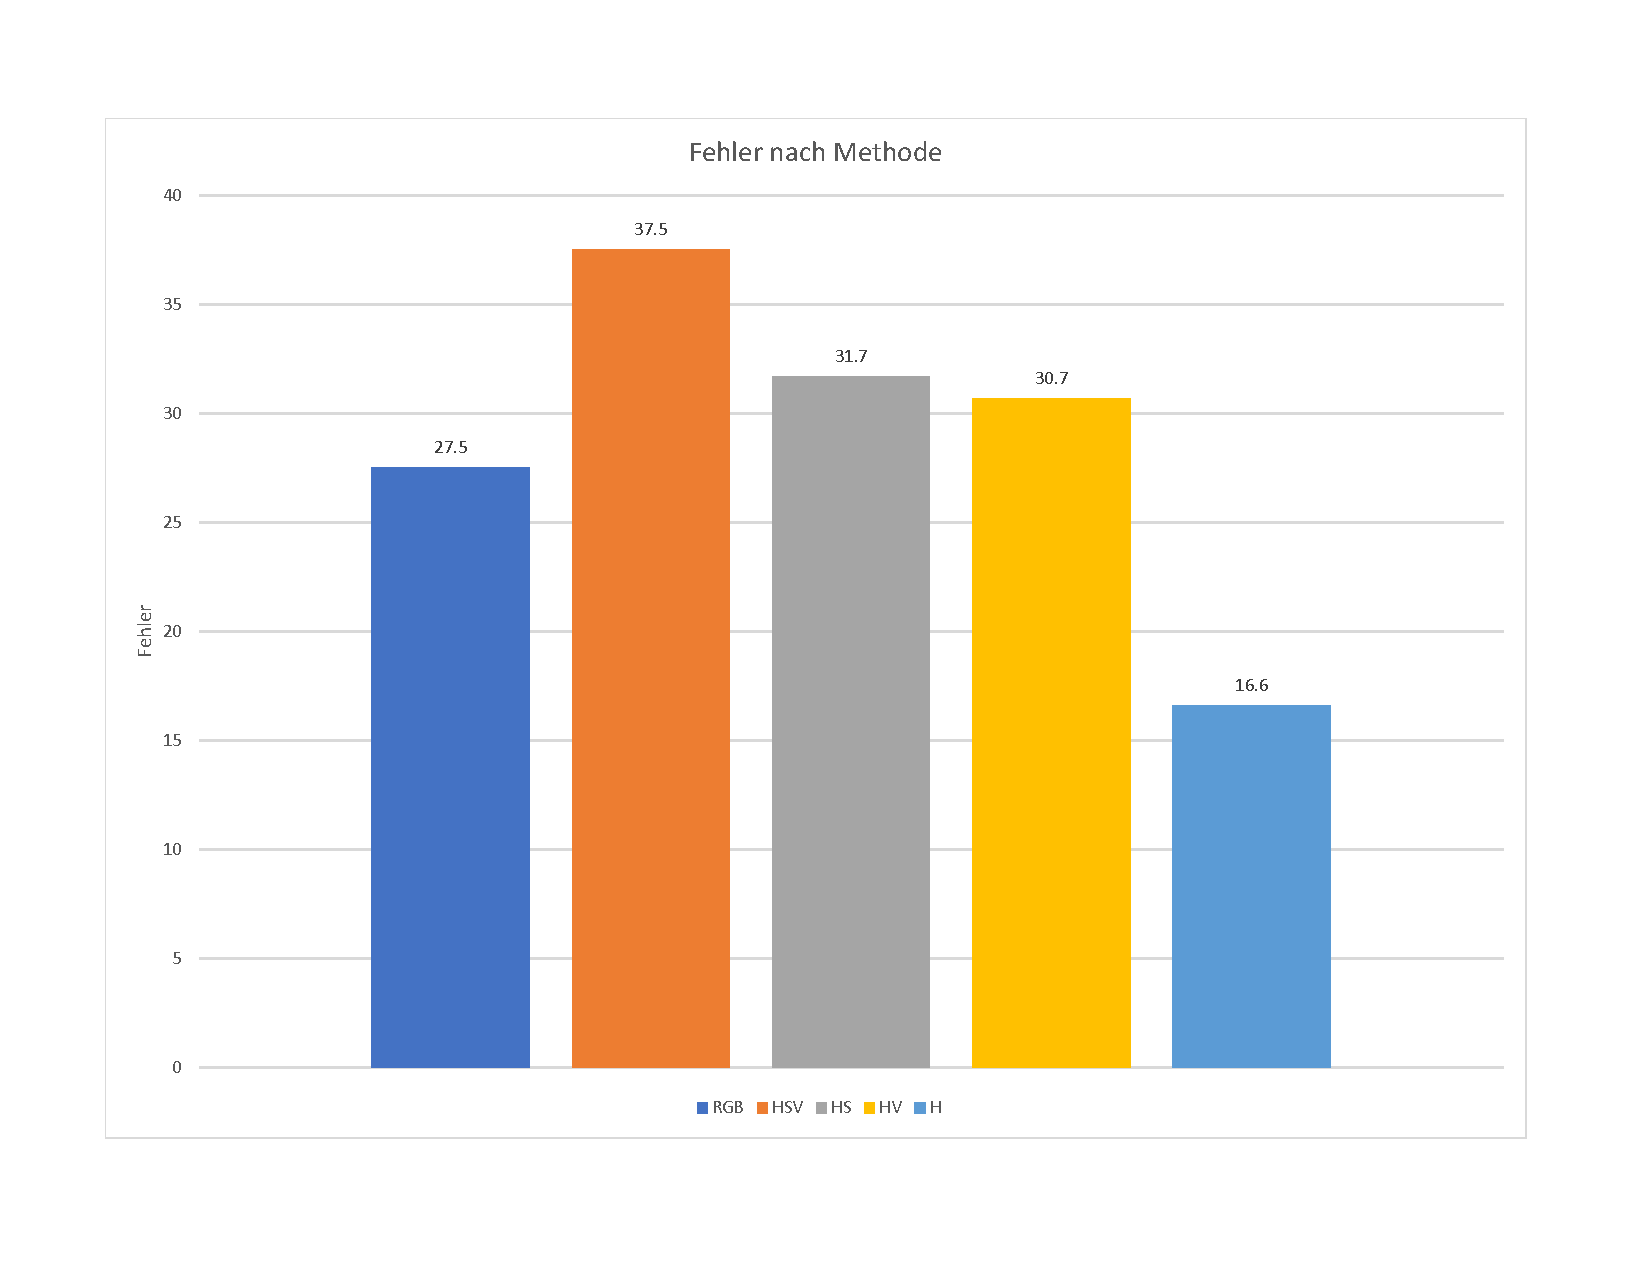
\includegraphics[scale=0.4]{Fehler_nach_Methode}
\caption{Durchschnittliche Anzahl Fehler für verschiedene Farbräume.}
\end{figure}
Wie im obigen Diagramm zu sehen, lieferte die Methode 5 die besten Ergebnisse, mit durchschnittlich 16.6 Fehlern bei 54 Feldern auf einem Würfel. Am zweitbesten war die RGB-Methode, mit jedoch fast doppelt so vielen Fehlern. Danach kamen nahe beieinander die Methoden 3 und 4, und schliesslich mit am meisten Fehlern die Methode 2. Dass die Methoden, die Saturation und/oder Value verwendeten, schlechter abschnitten, wie wenn nur Hue verwendet wurde war zu erwarten. Die Farben auf dem Würfel sind abgesehen von Weiss alle sehr satt und brillant. Wenn nun auf dem Bild eine Seite leicht überbelichtet oder schattig ist, dann verändert sich die Saturation oder der Value des Pixels. Somit werden dann zwei eigentlich identisch-farbige Felder als unterschiedlich angesehen, nur weil die Beleuchtung nicht identisch war. Diese Unterschiede werden bei Methode 5 nicht berücksichtigt, da nur die Hue-Werte verglichen werden. Auch die RGB-Methode erhält auf diese Weise Fehler. Da diese keine dedizierten Variablen für Sättigung und Helligkeit haben, verändern sich alle drei Variablen, wenn ein Feld andere Belichtung hat. Da sich diese Veränderung aber auf drei Variablen aufteilt, sind die einzelnen Werte nicht so weit entfernt, wie die von Saturation und Value. Und da die Quadrate der Entfernungen addiert werden, wirken sich zwei sehr falsche Werte mehr aus, als drei leicht falsche Werte. 
\begin{figure}[H]
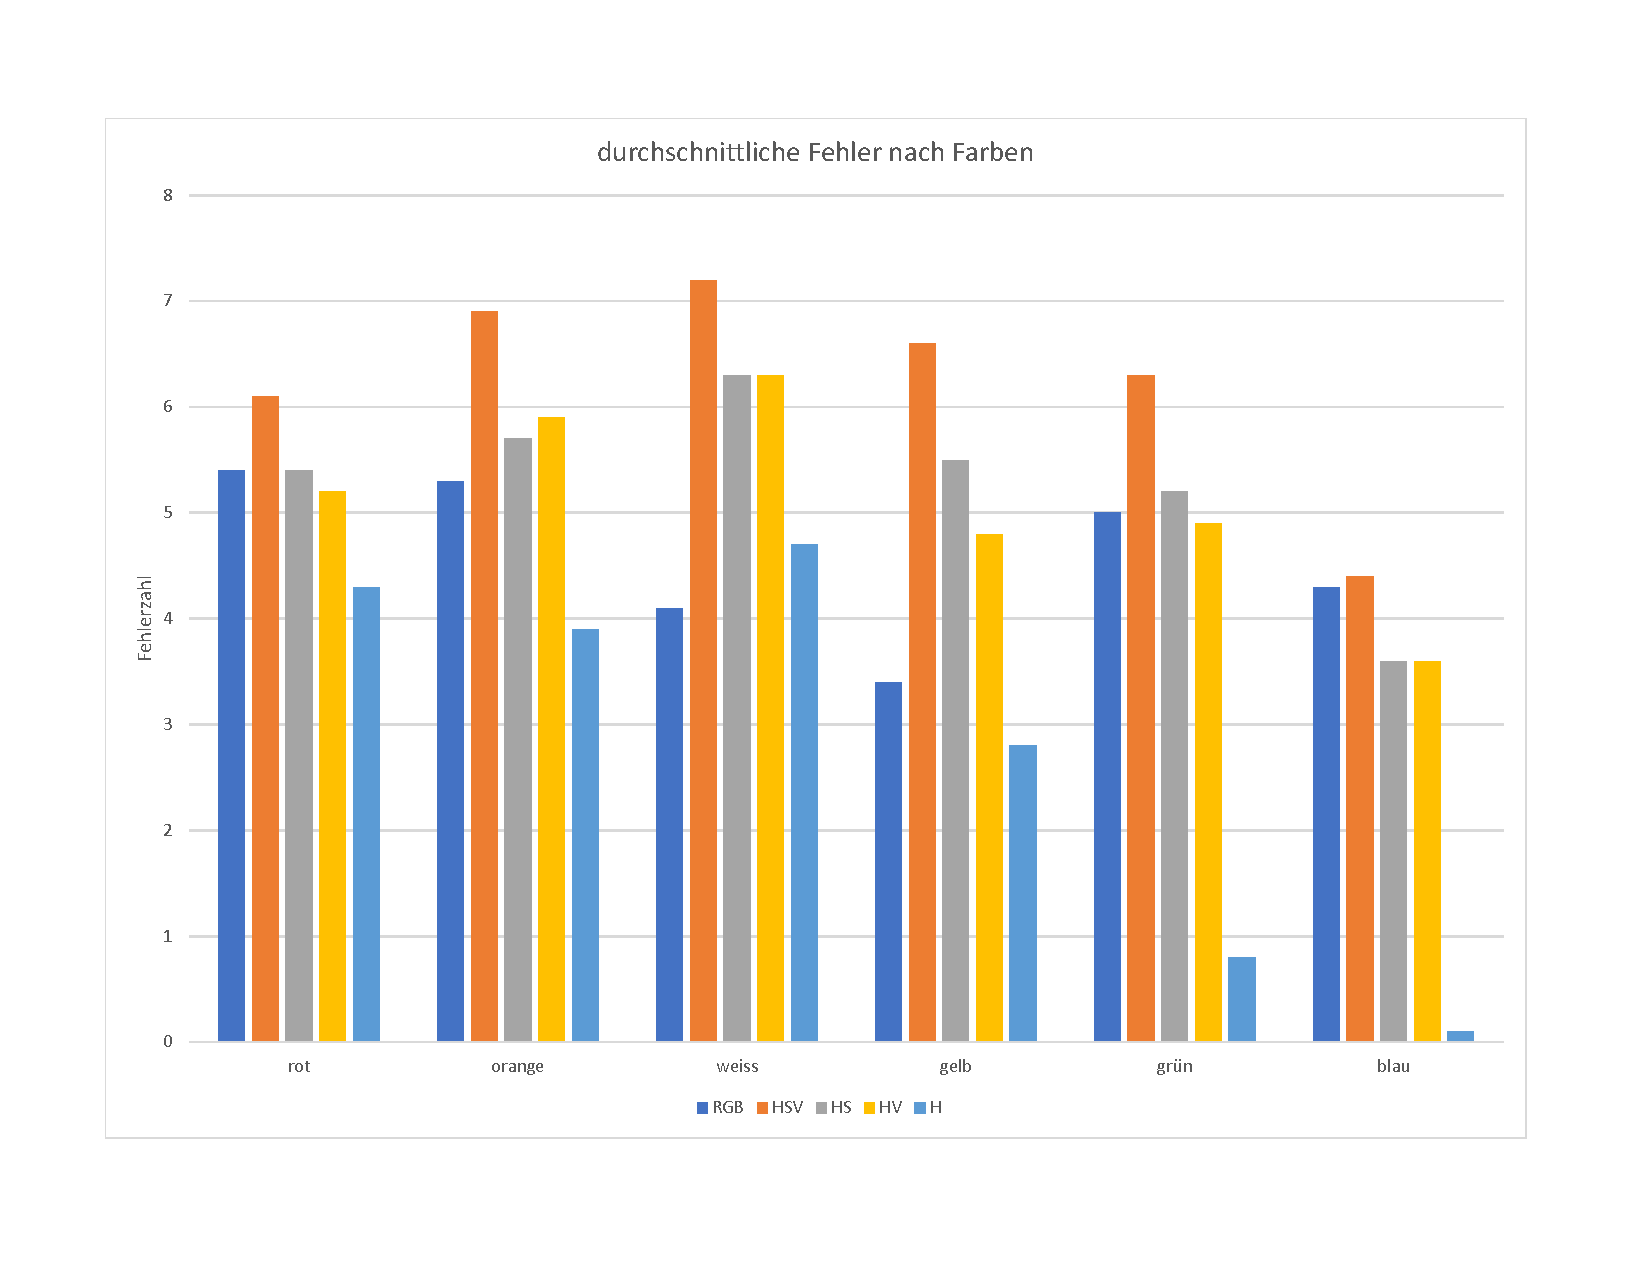
\includegraphics[scale=0.4]{durchschnittliche_Fehler_nach_Farben}
\caption{Durchschnittliche Anzahl Fehler für die verschiedenen Farbräume, aufgeteilt nach den einzelnen Farben.}
\end{figure}
Wenn man die Fehler nun nach Farben aufteilt, sieht man, dass die Methode 5 bei allen Farben die beste ist, ausser bei Weiss, wo RGB besser funktioniert. Dies lässt sich dadurch erklären, dass Weiss im HSV-Farbraum dann entsteht, wenn die Saturation 0 ist. Wenn etwas also komplett weiss ist, dann bedeutet dies, dass der Hue-Wert nicht definierbar ist. Das Programm erkennt somit einen zufälligen Farbton, wenn es ein weisses Feld erkennen muss. Das Programm hat somit keine richtige Möglichkeit, die weissen Felder nur anhand des Farbtons zuzuordnen, weshalb es dort zu überdurchschnittlich vielen Fehlern kommt. 
\subsection{Saturation/Value weg}
\subsubsection{Problem}
Wie im letzten Abschnitt erwähnt, ergibt sich, wenn nur Hue zur Unterscheidung der Farben verwendet wird, das Problem, dass wenn die Saturation einer Farbe sehr tief ist, die Hue-Werte fast nicht erkannt werden können. Das gleiche gilt auch für zu tiefe Value-Werte. Diese Felder müssen also auf eine andere Weise bestimmt werden. 
\subsubsection{Lösung}
Dieses Problem kann behoben werden, indem die weissen und die (falls vorhandenen) schwarzen Felder schon aussortiert werden, bevor die restlichen Felder einer Mitte zugeordnet werden. Zuerst werden alle Felder durchgegangen und es wird geschaut, ob sie einen festgelegten tiefen Saturation- oder Value-Wert unterschreiten.
\lstinputlisting[language=Python, linerange={23-26}, caption={Test, ob Seite eine tiefe Saturation oder einen tiefen Value hat.}, captionpos=b]{listings.py}
Danach wird geschaut, ob exakt 9 Felder einen tiefen Value-Wert besitzen. Ist dies der Fall, werden die Value-Werte der Mitten in den Zeilen 2 bis 5 verglichen, und die Mitte mit dem tiefsten Wert wird als schwarz festgelegt. Das gleiche Verfahren wird dann noch für das Ermitteln der 8 schwarzen Seiten angewendet (nicht im Listing abgebildet). Falls es nicht exakt 9 Felder mit einem tiefen Value Wert hat, aber trotzdem einige Felder als schwarz erkannt worden sind, bricht das Programm in Zeile 8 ab und gibt einen Error aus, da der Würfel dann nicht verlässlich erkannt werden kann. 
\lstinputlisting[language=Python, linerange={30-39}, caption={Methode, um die schwarze Mitte zu ermitteln.}, captionpos=b]{listings.py}
 Nachdem die schwarzen Felder aussortiert worden sind, wird analog das gleiche Verfahren für die Felder mit einer tiefen Saturation angewendet. Dabei muss noch beachtet werden, dass diejenigen Felder, bei denen die Saturation und der Value sehr tief sind, als schwarz erscheinen. Somit sind diese schon aussortiert worden und dürfen nicht mehr beachtet werden. 
\begin{figure}[H]
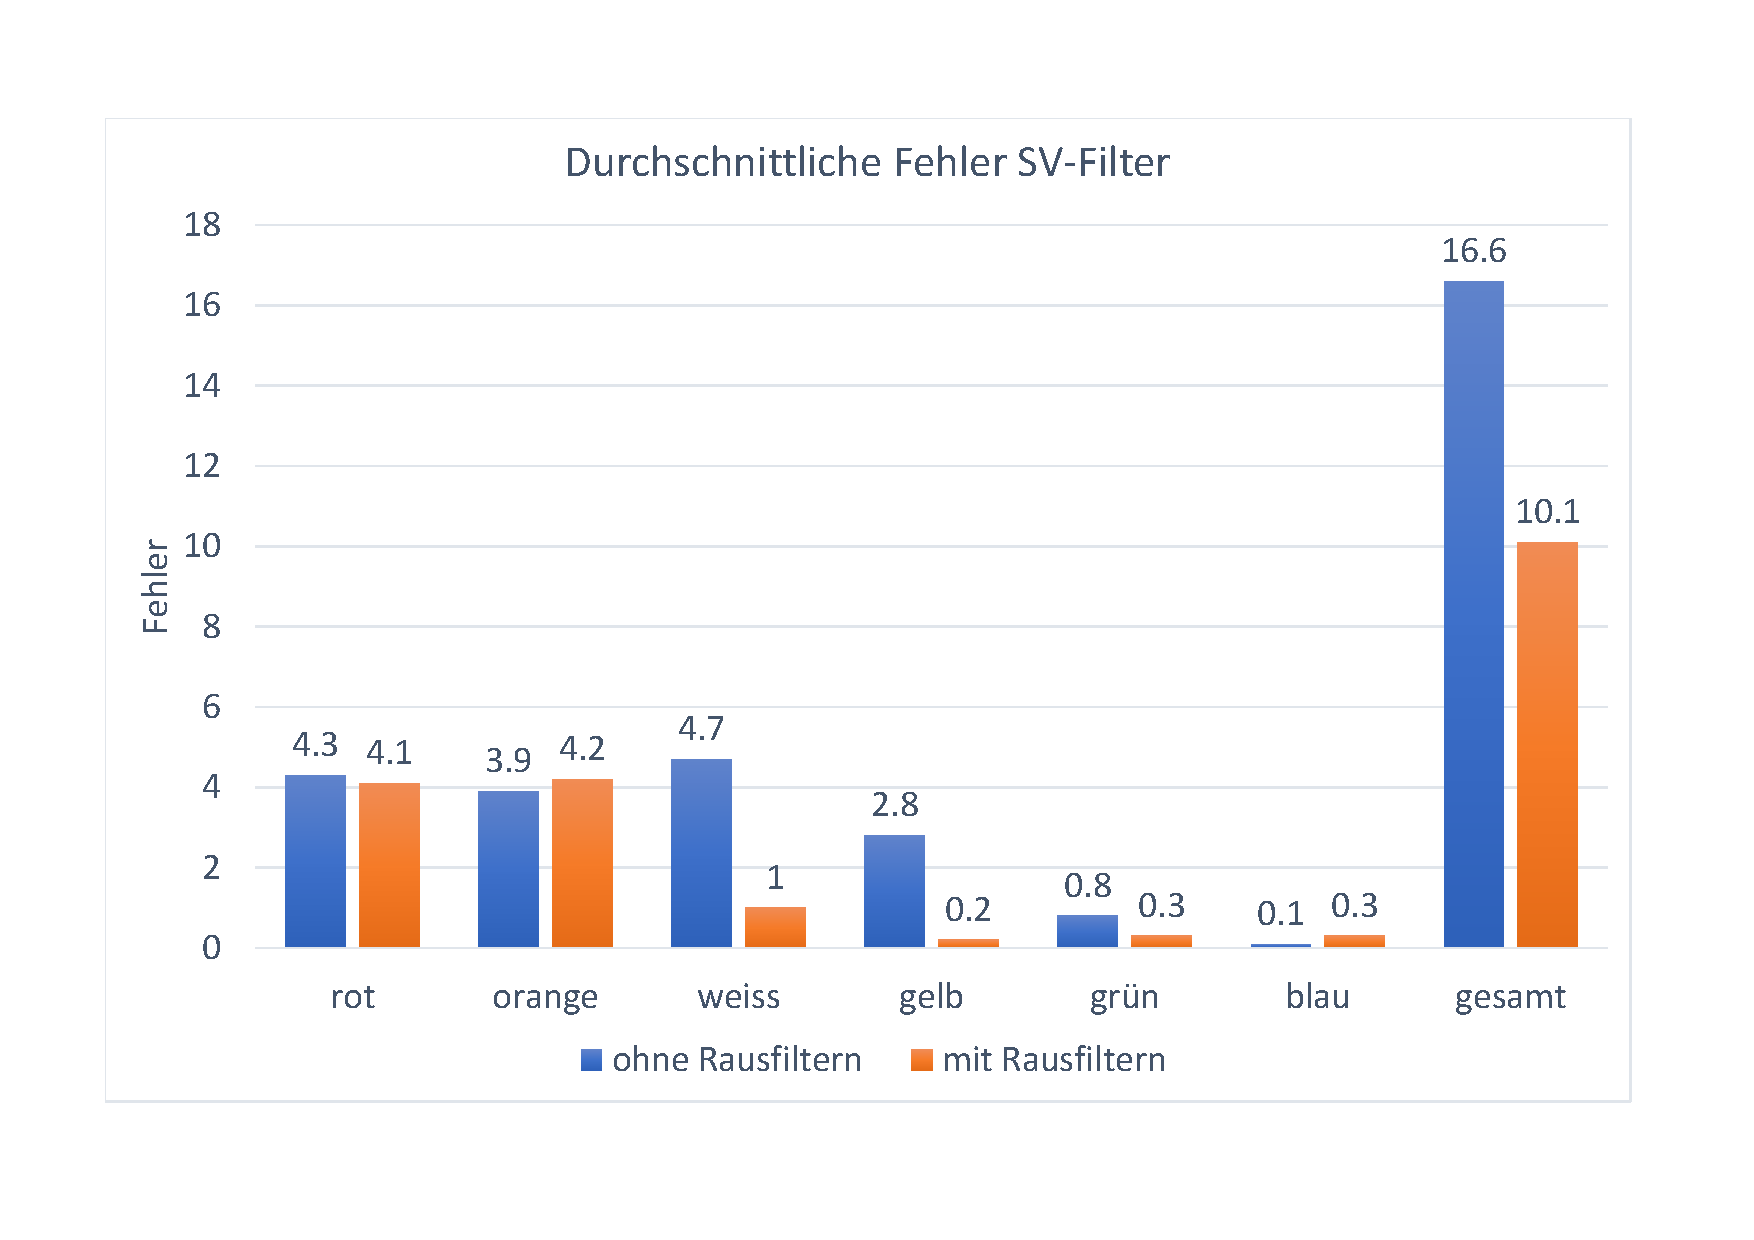
\includegraphics[scale=0.4]{Fehler_SV_Filter} 
\caption{Durchschnittliche Anzahl Fehler unter Anwenden des SV-Filters und ohne Anwenden des SV-Filters.}
\end{figure}
Durch das Anwenden dieser Filter, sinkt die durchschnittliche Fehlerzahl von 16.6 auf 10.1 Fehler auf 54 Felder. Diese Verbesserung kommt hauptsächlich wegen den weissen und gelben Feldern zustande. Von den weissen Feldern wird neu nur noch eins statt 4.7 falsch erkannt, und bei den Gelben sind es statt 2.8 noch 0.2 Fehler.
\subsection{Richtige Anzahl Felder pro Farbe}
Da bei einem Rubiks Cube bekannt ist, dass jede Farbe exakt neun mal vorkommt, weiss man, dass jeder Mitte exakt acht Felder zugeordnet werden müssen. Ist dies nach der Zuordnung nicht der Fall, lässt sich daraus schliessen, dass der Würfel noch nicht korrekt erkannt ist. In so einem Fall kann man nun noch einen Algorithmus einfügen, der dafür sorgt, dass jede Farbe exakt neun mal vorkommt. Dafür wurden zwei verschiedene Methoden ausprobiert.
\subsubsection{Nah an Mitte}
Die erste Methode ist die, die in den bisherigen Vergleichen auch schon angewendet worden ist. Falls einer Mitte zu viele Seiten zugeordnet wurden, sorgen die Schleifen in Zeilen 9 und 10 sowie die Bedingung in Zeile 11, dass diese Seiten alle mit den anderen Mitten verglichen werden. Dafür werden alle Abstände zwischen Seiten und Mitten auf zwei Bedingungen getestet. Die Erste ist, dass die Mitte weniger als 8 ihr zugeordnete Seiten haben muss. Die Zweite ist, dass der Abstand kleiner sein muss, wie der bisher kleinste gespeicherte Abstand. Ist dies der Fall, werden in den Zeilen 15 bis 18 der neue Abstand, die Farbe der Mitte und die Position der Seite gespeichert. Nachdem alle Abstände durchgelaufen sind, wird der gespeicherten Seite die neue Farbe zugewiesen, und die Anzahl Felder, die den Mitten zugeordnet sind, werden angepasst.
\lstinputlisting[language=Python, linerange={69-89}, caption={Korrekturmethode, bei der die Seiten, die am nächsten bei einer anderen Mitte sind, umgeordnet werden.}, captionpos=b]{listings.py}
\subsubsection{Weit weg von Mitte}
Der Beginn der zweiten Methode ist derselbe wie der, der ersten. Wenn einer Mitte zu viele Seiten zugeordnet wurden, werden  diese alle miteinander verglichen. Jedoch werden hier die Abstände zu der aktuell zugeordneten Mitte genommen, statt die Abstände zu den anderen Mitten. In der Zeile 10 wird geschaut, ob der Abstand zur eigenen Mitte der bisher grösste ist. Ist dies der Fall, werden in den Zeilen 11 bis 13 die Seite und der Abstand gespeichert. Wenn alle Seiten durch sind, wird diese mit dem grössten Abstand einer neuen Mitte zugeordnet. Dies geschieht in den Zeilen 14 bis 19 mit einem ähnlichen Prinzip wie in Methode 1. schliesslich werden in den Zeilen 20 und 21 noch die Variablen für die Anzahl zugeordnete Seiten angepasst.
\lstinputlisting[language=Python, linerange={44-64}, caption={Korrekturmethode, bei der die Felder, die am weitesten von der eigenen Mitte entfernt sind, umgeordnet werden.}, captionpos=b]{listings.py}
\subsubsection{Vergleich}
\begin{figure}[H]
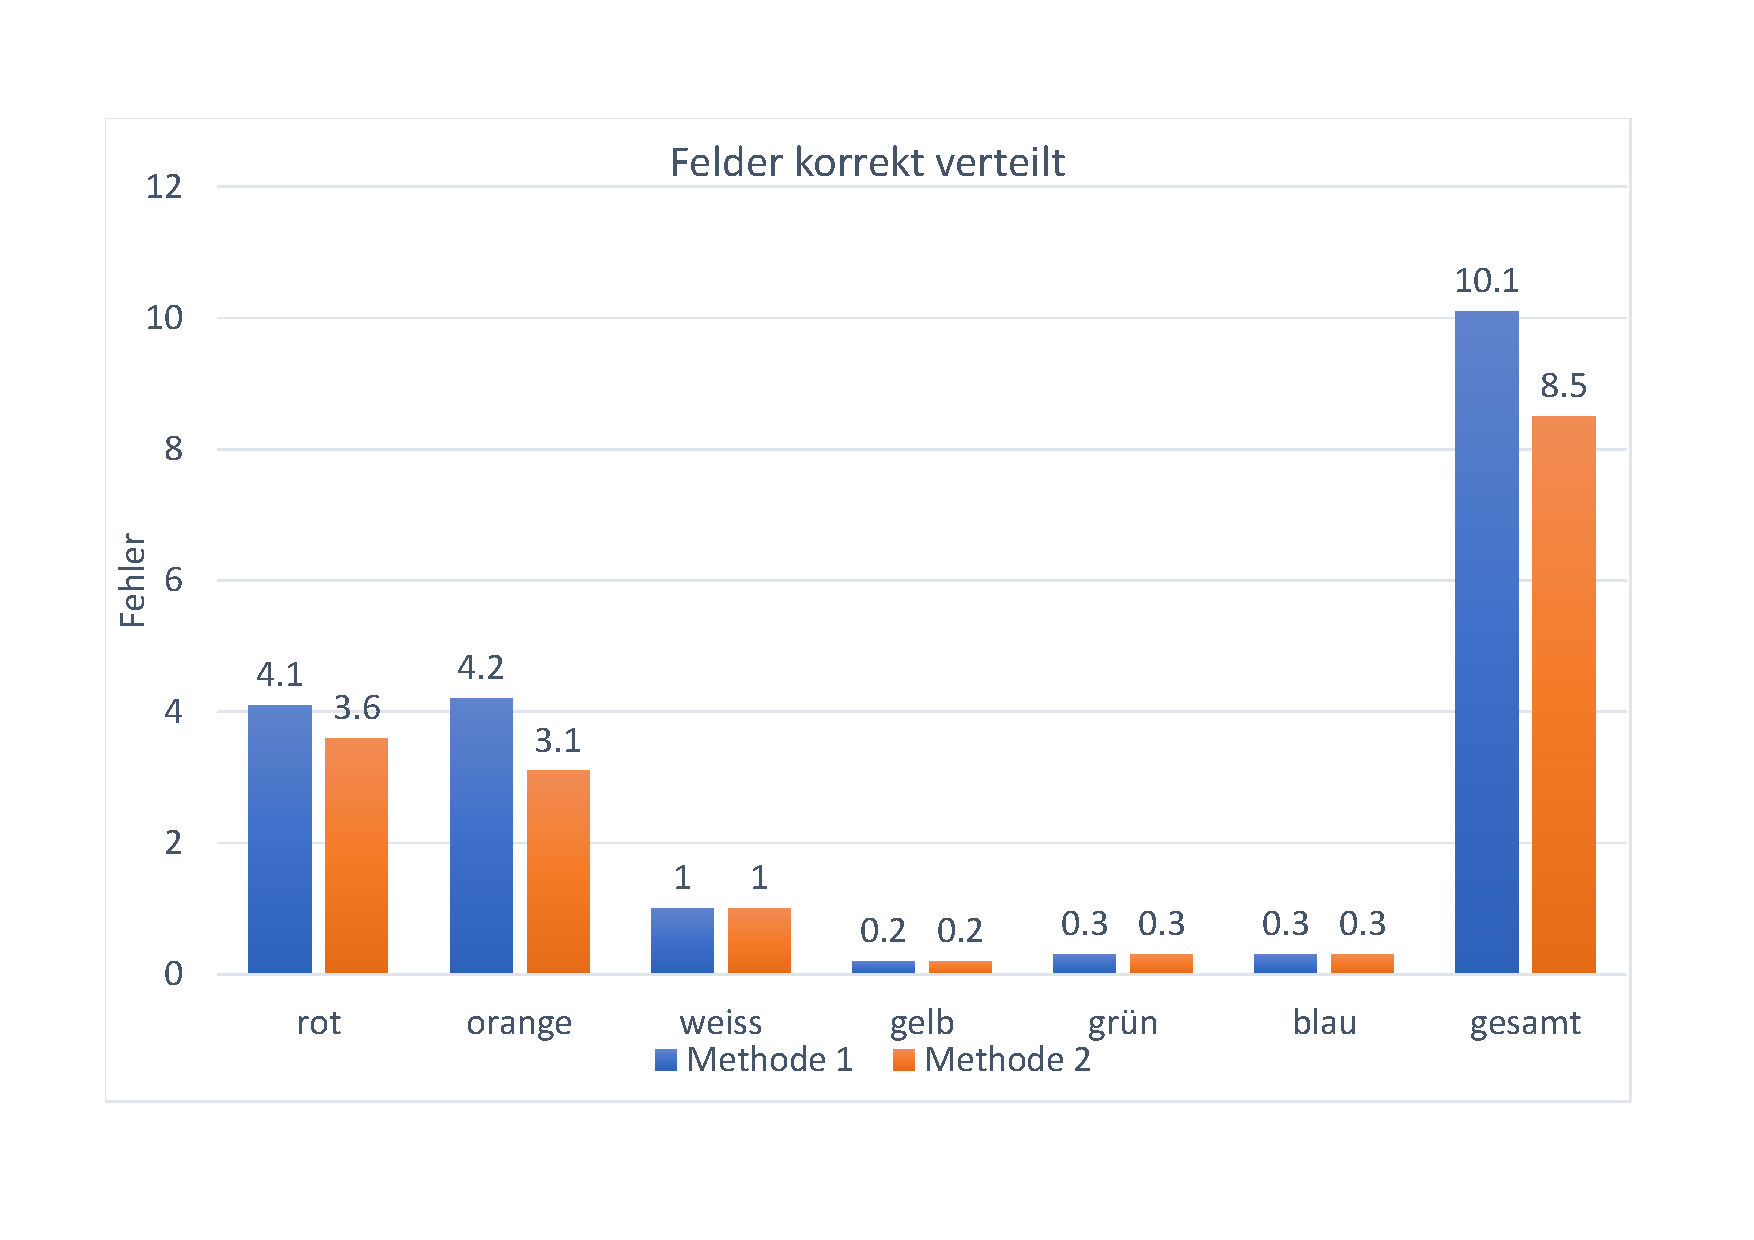
\includegraphics[scale=0.4]{Felder_korrekt_verteilt}
\caption{Durchschnittliche Anzahl Fehler, wenn eine der beiden Korrekturmethoden angewendet wird.}
\end{figure}
Wie im Diagramm zu sehen liefert die Methode 2 die besseren Resultate. Der Unterschied kommt jedoch nur bei den roten und orangen Feldern zustande. Bei allen anderen Farben sind die beiden Methoden gleich gut. 
\newpage
\section{Schluss}
Um hier noch einmal die Resultate zusammenzufassen: Es war immer ziemlich deutlich, welche Ideen besser waren, wie die anderen. Die besten Ergebnisse kamen heraus, wenn zuerst die weissen und schwarzen Felder herausgefiltert werden, danach die Felder anhand des Hue-Wertes zugeordnet werden, und dann schliesslich bei denen Farben, denen zu viele Felder zugeordnet wurden, die Felder, die am weitesten von der Mitte entfernt sind, noch umgeordenet werden. Aber auch dann gibt es im Schnitt noch 8.5 Fehler. Dies zeigt, dass es sehr schwierig ist, ein verlässliches Programm zu erstellen, welches den Rubiks Cube perfekt erkennt. Ein grosser Faktor, der dabei eine wichtige Rolle spielt, sind die Lichtverhältnisse. wenn die verschiedenen Seiten auch nur schon einen kleinen Unterschied in der Beleuchtung haben, kann es zu Fehlern kommen. Es wird versucht, diese zu minimieren, indem nur Hue als Unterscheidungsmerkmal verwendet wird, aber es entstehen trotzdem noch Fehler. Eine andere grosse Fehlerquelle ist das Unterscheiden von rot und orange. Da diese einen sehr ähnlichen Hue-Wert haben, ist es schwierig sie unterscheiden zu können und schon minimale Störungen im Bild können zu falschen Resultaten führen. Es gibt aber noch einige Ideen, die die Anzahl Fehler möglicherweise noch reduzieren könnten. Zum Beispiel könnte noch geschaut werden, ob das erkannte Muster überhaupt entstehen kann, wenn ein Rubiks Cube vermischt wird. Es ist beispielsweise nicht möglich, dass auf einem Eckstein eine Farbe mehrmals vorkommt. Es kann auch noch weiter erforscht werden, wie die Veränderung der Lichtverhältnisse die erkannten Farben verändert. Es wäre auch möglich einen komplett anderen Ansatz zu versuchen, indem man ein neuronales Netz verwendet. Hier käme einfach das Problem hinzu, dass das Trainieren eines neuronalen Netzes, möglicherweise hunderte oder tausende von Bildern benötigt, was sehr aufwendig wäre.
\newpage
\printbibliography[heading=bibnumbered]
\end{document}
